\documentclass[table]{beamer}
%\documentclass[table]{beamer}
%[]中可以使用draft、handout、screen、transparency、trancompress、compress等参数

%指定beamer的模式与主题
\mode<presentation>
{
  \usetheme{Madrid}
%\usetheme{Boadilla}
%\usecolortheme{default}
%\usecolortheme{orchid}
%\usecolortheme{whale}
%\usefonttheme{professionalfonts}
}

%\usetheme{Madrid}
%这里还可以选择别的主题:Bergen, Boadilla, Madrid, AnnArbor, CambridgeUS, Pittsburgh, Rochester, Warsaw, ...
%有导航栏的Antibes, JuanLesPins, Montpellier, ...
%有内容的Berkeley, PaloAlto, Goettingen, Marburg, Hannover, ...
%有最小导航栏的Berlin, Ilmenau, Dresden, Darmstadt, Frankfurt, Singapore, Szeged, ...
%有章和节表单的Copenhagen, Luebeck, Malmoe, Warsaw, ...

%\usecolortheme{default}
%设置内部颜色主题(这些主题一般改变block里的颜色);这个主题一般选择动物来命名
%这里还可以选择别的颜色主题,如默认的和有特别目的的颜色主题default,structure,sidebartab,全颜色主题albatross,beetle,crane,dove,fly,seagull,wolverine,beaver

%\usecolortheme{orchid}
%设置外部颜色主题(这些主题一般改变title里的颜色);这个主题一般选择植物来命名
%这里还可以选择别的颜色主题,如默认的和有特别目的的颜色主题lily,orchid,rose

%\usecolortheme{whale}
%设置字体主题;这个主题一般选择海洋动物来命名
%这里还可以选择别的颜色主题,如默认的和有特别目的的颜色主题whale,seahorse,dolphin

%\usefonttheme{professionalfonts}
%类似的还可以定义structurebold,structuresmallcapsserif,professionalfonts


% 控制 beamer 的风格,可以根据自己的爱好修改
%\usepackage{beamerthemesplit} %使用 split 风格
%\usepackage{beamerthemeshadow} %使用 shadow 风格
%\usepackage[width=2cm,dark,tab]{beamerthemesidebar}


% 设定英文字体
%\usepackage{fontspec}
\usepackage[no-math]{fontspec}
\setmainfont{Times New Roman}
\setsansfont{Arial}
\setmonofont{Courier New}

% 设定中文字体
\usepackage[BoldFont,SlantFont,CJKchecksingle,CJKnumber]{xeCJK}
%\setCJKmainfont[BoldFont={Adobe Heiti Std},ItalicFont={Adobe Kaiti Std}]{Adobe Song Std}
\setCJKmainfont[BoldFont={Adobe Heiti Std},ItalicFont={Adobe Kaiti Std}]{WenQuanYi Micro Hei}
\setCJKsansfont{Adobe Heiti Std}
\setCJKmonofont{Adobe Fangsong Std}
\punctstyle{hangmobanjiao}

\defaultfontfeatures{Mapping=tex-text}
\usepackage{xunicode}
\usepackage{xltxtra}

\XeTeXlinebreaklocale "zh"
\XeTeXlinebreakskip = 0pt plus 1pt minus 0.1pt

\usepackage{setspace}
\usepackage{colortbl,xcolor}
\usepackage{hyperref}
%\hypersetup{xetex,bookmarksnumbered=true,bookmarksopen=true,pdfborder=1,breaklinks,colorlinks,linkcolor=blue,filecolor=black,urlcolor=cyan,citecolor=green}
\hypersetup{xetex,bookmarksnumbered=true,bookmarksopen=true,pdfborder=1,breaklinks,colorlinks,linkcolor=cyan,filecolor=black,urlcolor=blue,citecolor=green}

% 插入图片
\usepackage{graphicx}
\graphicspath{{figures/}}

% 可能用到的包
\usepackage{amsmath,amssymb}
\usepackage{multimedia}
\usepackage{multicol}
\usepackage{multirow}

% 定义一些自选的模板,包括背景、图标、导航条和页脚等,修改要慎重
% 设置背景渐变由10%的红变成10%的结构颜色
%\beamertemplateshadingbackground{red!10}{structure!10}
%\beamertemplatesolidbackgroundcolor{white!90!blue}
% 使所有隐藏的文本完全透明、动态,而且动态的范围很小
\beamertemplatetransparentcovereddynamic
% 使itemize环境中变成小球,这是一种视觉效果
\beamertemplateballitem
% 为所有已编号的部分设置一个章节目录,并且编号显示成小球
\beamertemplatenumberedballsectiontoc
% 将每一页的要素的要素名设成加粗字体
\beamertemplateboldpartpage

% item逐步显示时,使已经出现的item、正在显示的item、将要出现的item呈现不同颜色
\def\hilite<#1>{
 \temporal<#1>{\color{gray}}{\color{blue}}
    {\color{blue!25}}
}

\renewcommand{\today}{\number\year 年 \number\month 月 \number\day 日}

%五角星
\usepackage{MnSymbol}

%去除图表标题中的figure等
\usepackage{caption}
\captionsetup{labelformat=empty,labelsep=none}

\usepackage{tabu}
\usepackage{multirow}

% 千分号
%\usepackage{textcomp}

%罗马数字
\makeatletter
\newcommand{\rmnum}[1]{\romannumeral #1}
\newcommand{\Rmnum}[1]{\expandafter\@slowromancap\romannumeral #1@}
\makeatother

%分栏
\usepackage{multicol}

%\usepackage{enumitem}
\usepackage{enumerate}


%\setbeamercolor{alerted text}{fg=magenta}

\setbeamercolor{bgcolor}{fg=yellow,bg=cyan}

\begin{document}

%\includeonlyframes{current}

\logo{\includegraphics[height=0.08\textwidth]{tijmu.png}}
\title[基因组功能注释分析]{基因组功能注释分析}
\author[Yixf]{伊现富(Yi Xianfu)}
\institute[TIJMU]{天津医科大学(TIJMU)\\ 生物医学工程学院}
\date{2014年4月}


% 在每个Section前都会加入的Frame
\AtBeginSection[]
{
  \begin{frame}<beamer>
    %\frametitle{Outline}
    \frametitle{教学提纲}
    \setcounter{tocdepth}{2}
    \begin{multicols}{2}
    %\tableofcontents[currentsection,currentsubsection]
    \tableofcontents[currentsection]
  \end{multicols}
  \end{frame}
}
% 在每个Subsection前都会加入的Frame
%\AtBeginSubsection[]
%{
  %\begin{frame}<beamer>
%%\begin{frame}<handout:0>
%% handout:0 表示只在手稿中出现
    %\frametitle{Outline}
    %\setcounter{tocdepth}{2}
    %\tableofcontents[currentsection,currentsubsection]
%% 显示在目录中加亮的当前章节
  %\end{frame}
%}

\begin{frame}[plain]
  \begin{center}
    {\Huge 生物信息学\\}
    \vspace{1cm}
    {\LARGE 天津医科大学\\}
    %\vspace{0.2cm}
    {\LARGE 生物医学工程学院\\}
    \vspace{1cm}
    {\large 2013-2014学年下学期(春)\\ 2011级生信班}
  \end{center}
\end{frame}

\begin{frame}
  \titlepage
\end{frame}

\begin{frame}[plain]
  \frametitle{教学提纲}
  \setcounter{tocdepth}{2}
  \begin{multicols}{2}
  \tableofcontents
  \end{multicols}
\end{frame}

\section{引言}
\begin{frame}
  \frametitle{基因组注释}
  \begin{block}{基因组注释(genome annotation)}
    \begin{itemize}
      \item 结构注释(structural annotation) $\Leftarrow$ 实验手段,单个基因
      \begin{itemize}
        \item 限制性酶切位点分析、开放阅读框分析、启动子分析、CpG岛识别
        \item 重复序列分析、基因识别
        \item mRNA选择性剪接分析
      \end{itemize}
      \item 功能注释(functional annotation) $\Leftarrow$ 组学时代,复杂疾病
      \begin{itemize}
        \item 变异位点的注释
        \item 基因集富集分析
        \item 生物学通路分析
        \item 相互作用网络分析
        \item 分子进化分析
      \end{itemize}
    \end{itemize}
  \end{block}
\end{frame}

\begin{frame}
  \frametitle{引言 | 基础知识}
  \begin{itemize}
    \item 基因组组装版本
    \item 基因组坐标系统
    \item 注释常用格式
    \item 文本编辑器
    \item 坐标的逻辑运算
  \end{itemize}
\end{frame}

\begin{frame}
  \frametitle{引言 | NGS}
  \begin{center}
    \includegraphics[width=10cm]{ngs.jpg}
  \end{center}
\end{frame}

\section{基因组组装版本}
\begin{frame}
  \frametitle{组装版本 | 疑惑}
  \begin{itemize}
    \item These sequences were mapped to human and mouse genomes sequences (\alert{hg18 and mm9}, respectively) using BLASTN.
    \item We used DNA sequences from the human and mouse genome assemblies \alert{hg18 and mm9}.
    \item Currently there are ~25,000 genes annotated in the human (\alert{hg18}) and mouse (\alert{mm9}) genome, which comprise less than 3\% of the genome (UCSC genome browser; http://genome.ucsc.edu/).
    \item The \alert{GRCh37/hg19 and GRCm38/mm10} assemblies at the UCSC genome browser (http://genome.ucsc.edu/) were used for mapping the chromosomal defect and gene annotations.
    \item The genome assemblies from which the sequences obtained were Dec 2011 (\alert{GRCm38/mm10}), Feb 2009 (\alert{GRCh37/hg19}) and Nov 2004 (\alert{Baylor3.4/rn4}) for mouse, human and rat respectively.
  \end{itemize}
\end{frame}


\begin{frame}
  \frametitle{组装版本 | XP vs. Win7}
  \begin{center}
    \includegraphics[width=9cm]{windows.jpg}
  \end{center}
\end{frame}

\begin{frame}
  \frametitle{组装版本 | 版本对照}
  \begin{center}
  \alert{基因组序列不是确定的吗?也需要版本升级?}
  \end{center}
  \pause
  \begin{table}
    \centering
    \rowcolors[]{1}{blue!20}{blue!10}
    \begin{tabular}{cccc}
      \hline
      \rowcolor{blue!50} SPECIES & UCSC & DATE & NCBI\\
      Human & hg19 & Feb. 2009 & Genome Reference Consortium\\
       & & & GRCh37\\
       & hg18 & Mar. 2006 & NCBI Build 36.1\\
       & hg17 & May 2004 & NCBI Build 35\\
       & hg16 & Jul. 2003 & NCBI Build 34\\
      \hline
      Mouse & mm10 & Dec. 2011 & Genome Reference Consortium\\
       & & & GRCm38\\
       & mm9 & Jul. 2007 & NCBI Build 37\\
       & mm8 & Feb. 2006 & NCBI Build 36\\
       & mm7 & Aug. 2005 & NCBI Build 35\\
      \hline
    \end{tabular}
  \end{table}
  \pause
  \begin{center}
    human: \textit{Homo sapiens}; mouse: \textit{\alert{M}us \alert{m}usculus}

    hg: \alert{h}uman \alert{g}enome; GRC: \alert{G}enome \alert{R}eference \alert{C}onsortium
  \end{center}
\end{frame}

\section{基因组坐标系统}
\begin{frame}
  \frametitle{坐标系统 | 坐标轴}
  \only<1,2>{
  \begin{center}
    \includegraphics[width=6cm]{2d.png}
  \end{center}
  }
  \pause
  \only<2,3>{
  \begin{center}
    \includegraphics[width=9cm]{1d.png}
  \end{center}
  }
  \pause
  \only<3,4>{
  \begin{center}
    \includegraphics[width=7cm]{dna.png}
  \end{center}
  }
  \pause
  \only<4>{
  \begin{block}{hg19}
    \begin{itemize}
      \item SNP, rs1800468: ''chr19\ \ \ 41860587''; ''chr19:41860587''
      \item gene, \textit{SAMD11}: ''chr1 \ \ \ 861121\ \ \ 879961''; ''chr1:861121-879961''
    \end{itemize}
  \end{block}
  }
\end{frame}

\begin{frame}
  \frametitle{坐标系统 | 两大系统}
  \begin{block}{序列}
  \begin{table}
    \centering
    \rowcolors[]{1}{blue!20}{blue!10}
    \begin{tabular}{lcccccccc}
      \hline
      0-based index & 0 & 1 & 2 & 3 & 4 & 5 & 6 & 7\\
      \hline
      Sequence & A & A & T & T & G & G & C & C\\
      \hline
      1-based index & 1 & 2 & 3 & 4 & 5 & 6 & 7 & 8\\
      \hline
    \end{tabular}
  \end{table}
  \end{block}
  \pause
  \begin{block}{TG的坐标}
    \begin{itemize}
      \item 0-based,half-open:[3,5)
      \item 1-based,fully-closed:[4,5]
    \end{itemize}
  \end{block}
  \pause
  \begin{block}{实例}
    \begin{itemize}
      \item 0-based:BED、BAM、PSL,dbSNP、Table Browser
      \item 1-based:GFF、VCF、SAM、Wiggle,DAS、Genome Browser
    \end{itemize}
  \end{block}
\end{frame}

\begin{frame}
  \frametitle{坐标系统 | 类比}
  \begin{columns}
  \column{0.5\textwidth}
  \visible<1->{
  \begin{block}{first floor}
    \begin{center}
      \includegraphics[width=6cm]{firstFloor.jpg}
    \end{center}
  \end{block}
  }
  \column{0.48\textwidth}
  \visible<2->{
  \begin{block}{数组}
    \begin{center}
      \includegraphics[width=5.5cm]{array.png}
    \end{center}
  \end{block}
  }
  \end{columns}
\end{frame}

\section{基因组注释常用格式}
\begin{frame}
  \frametitle{格式 | 文件格式}
    \begin{center}
      \includegraphics[width=7cm]{format.jpg}
    \end{center}
\end{frame}

\begin{frame}
  \frametitle{格式 | FASTA}
    \begin{center}
      \includegraphics[width=12cm]{fasta.png}
    \end{center}
\end{frame}

\begin{frame}
  \frametitle{格式 | FASTA | 注意事项}
  \begin{itemize}
    \item 每一行最好不要超过80个字符
    \item 序列中的换行符不会影响序列的连续性
    \item 使用标准的IUB/IUPAC核酸代码和氨基酸代码
    \item 允许小写字母的存在,但会转换成大写
    \item 单个“-”代表不明长度的空位
    \item 在氨基酸序列中允许出现“U”和“*”
    \item 任何数字都应该被去掉或转换成字母
    \item 不明核酸和氨基酸分别用“N”和“X”表示
  \end{itemize}
\end{frame}

\begin{frame}
  \frametitle{格式 | FASTA | IUB/IUPAC核酸}
    \begin{center}
      \includegraphics[width=8cm]{iub.png}
    \end{center}
\end{frame}

\begin{frame}
  \frametitle{格式 | FASTA | IUB/IUPAC核酸}
    \begin{center}
      \includegraphics[width=12cm]{na.png}
    \end{center}
\end{frame}

\begin{frame}
  \frametitle{格式 | FASTA | IUB/IUPAC氨基酸}
    \begin{center}
      \includegraphics[width=11cm]{aa.png}
    \end{center}
\end{frame}

\begin{frame}
  \frametitle{格式 | FASTA | FASTA vs. Sequence}
  \begin{block}{FASTA}
    \begin{center}
      \includegraphics[width=12cm,height=4cm]{fasta.png}
    \end{center}
  \end{block}
  \begin{block}{Sequence}
    \begin{itemize}
      \item {\scriptsize GTACGACGGAGTGTTATAAGATGGGAAATCGGATACCAGATGAAATTGTGGATCAG}
      \item {\scriptsize MWTALPLLCAGAWLLSAGATAELTVNAIEKFHFTSWMKQHQKTYSSREYSHRLQVFAN}
    \end{itemize}
  \end{block}
\end{frame}

\begin{frame}
  \frametitle{格式 | BED (Browser Extensible Data)}
    \begin{center}
      \includegraphics[width=12cm,height=5.5cm]{bed.png}
    \end{center}
\end{frame}

\begin{frame}
  \frametitle{格式 | BED\#}
  \begin{block}{BED\#}
  \begin{description}
    \item[BED12]<alert@1> 包含全部12列
    \item[BED6]<alert@2> chrom, start, end, name, score, and strand
    \item[BED5]<alert@3> chrom, start, end, name, and score
    \item[BED4]<alert@4> chrom, start, end, and name
    \item[BED3]<alert@5> chrom, start, and end
  \end{description}
\end{block}
\begin{block}{例子}
    \only<1>{chr1\ \ \ \ \ 11873\ \ \ \ \ 14409\ \ \ \ \ uc001aaa.3\ \ \ \ \ 0\ \ \ \ \ +\ \ \ \ \ 11873\ \ \ \ \ 11873\ \ \ \ \ 0\ \ \ \ \ 3\ \ \ \ \ 354,109,1189,\ \ \ \ \ 0,739,1347,}
    \only<2>{chr1\ \ \ \ \ 11873\ \ \ \ \ 14409\ \ \ \ \ uc001aaa.3\ \ \ \ \ 0\ \ \ \ \ +}
    \only<3>{chr1\ \ \ \ \ 11873\ \ \ \ \ 14409\ \ \ \ \ uc001aaa.3\ \ \ \ \ 0}
    \only<4>{chr1\ \ \ \ \ 11873\ \ \ \ \ 14409\ \ \ \ \ uc001aaa.3}
    \only<5>{chr1\ \ \ \ \ 11873\ \ \ \ \ 14409}
  \end{block}
\end{frame}

\begin{frame}
  \frametitle{格式 | GFF (General Feature Format)}
    \begin{center}
      \includegraphics[width=12cm,height=4.5cm]{gff.png}
    \end{center}
\end{frame}

\begin{frame}
  \frametitle{格式 | VCF (Variant Call Format)}
    \begin{center}
      \includegraphics[width=12cm,height=5.5cm]{vcf.png}
    \end{center}
\end{frame}

\section{文本文件与文本编辑器}
\begin{frame}
  \frametitle{文本 | 纯文本 vs. 格式化文本}
    \begin{center}
      \includegraphics[width=5.9cm,height=6.45cm]{txt.png}
      \vspace*{0.1cm}
      \includegraphics[width=6cm]{word.png}
    \end{center}
\end{frame}

\begin{frame}[fragile]
  \frametitle{文本 | 换行符}
  \begin{block}{三大类}
    \begin{itemize}
      \item Windows:\verb|\r\n|(CR+LF,回车+换行),文件尾部直接EOF(文件结束标志)
      \item Unix:\verb|\n|(LF,仅有换行),文件最后一行也会增加该字符,然后才是EOF
      \item Mac:\verb|\r|(CR,仅有回车)
    \end{itemize}
  \end{block}
  \pause
  \begin{block}{识别与转换}
    \begin{itemize}
      \item Windows:文本编辑器,如Notepad++
      \item Unix:file识别,fromdos \& todos转换
    \end{itemize}
  \end{block}
\end{frame}

\begin{frame}
  \frametitle{文本 | 编辑器}
    \begin{center}
      \includegraphics[width=9cm]{editor.png}
    \end{center}
\end{frame}

\begin{frame}
  \frametitle{文本 | 编辑器 | Notepad++}
    \begin{center}
      \includegraphics[width=10cm]{notepad.png}
    \end{center}
\end{frame}

\begin{frame}
  \frametitle{文本 | 编辑器 | Vim}
    \begin{center}
      \includegraphics[width=10cm]{vim.jpg}
    \end{center}
\end{frame}

\begin{frame}
  \frametitle{文本 | 编辑器 | Emacs}
    \begin{center}
      \includegraphics[width=8cm]{emacs.png}
    \end{center}
\end{frame}

\begin{frame}
  \frametitle{文本 | 编辑器 | Sublime Text}
    \begin{center}
      \includegraphics[width=11cm]{sublime.png}
    \end{center}
\end{frame}

\section{基因组坐标的逻辑运算}
\begin{frame}
  \frametitle{逻辑运算 | 集合运算}
    \begin{center}
      \includegraphics[width=9cm]{set.png}
    \end{center}
\end{frame}

\begin{frame}
  \frametitle{逻辑运算 | 集合 $\Rightarrow$ 基因组}
    \begin{center}
      \includegraphics[width=9cm]{setT.png}
    \end{center}
\end{frame}

\begin{frame}
  \frametitle{逻辑运算 | 运算模式}
    \begin{center}
      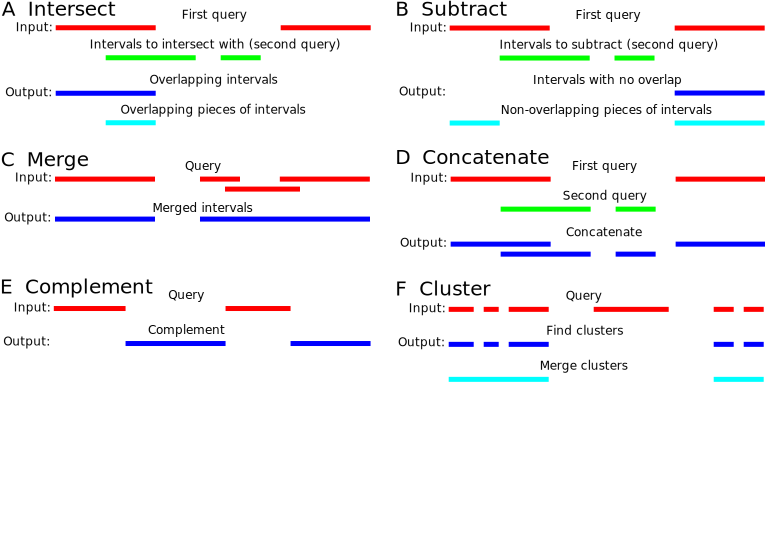
\includegraphics[width=11cm]{operation.png}
    \end{center}
\end{frame}

\begin{frame}
  \frametitle{逻辑运算 | intersect}
    \begin{center}
      \includegraphics[width=11cm]{intersect.png}
    \end{center}
\end{frame}

\begin{frame}
  \frametitle{逻辑运算 | intersect}
    \begin{center}
      \includegraphics[width=11cm]{intersectA.png}
      \vspace{0.5cm}
      \includegraphics[width=11cm]{intersectB.png}
    \end{center}
\end{frame}

\begin{frame}
  \frametitle{逻辑运算 | subtract}
    \begin{center}
      \includegraphics[width=11cm]{subtract.png}
    \end{center}
\end{frame}

\begin{frame}
  \frametitle{逻辑运算 | subtract}
    \begin{center}
      \includegraphics[width=11cm]{subtractA.png}
      \vspace{0.5cm}
      \includegraphics[width=11cm]{subtractB.png}
    \end{center}
\end{frame}

\begin{frame}
  \frametitle{逻辑运算 | merge}
    \begin{center}
      \includegraphics[width=11cm]{merge.png}
    \end{center}
\end{frame}

\begin{frame}
  \frametitle{逻辑运算 | merge}
    \begin{center}
      \includegraphics[width=11cm]{mergeA.png}
      \vspace{0.5cm}
      \includegraphics[width=11cm]{mergeB.png}
    \end{center}
\end{frame}

\begin{frame}
  \frametitle{逻辑运算 | concatenate}
    \begin{center}
      \includegraphics[width=11cm]{concatenate.png}
    \end{center}
\end{frame}

\begin{frame}
  \frametitle{逻辑运算 | complement}
    \begin{center}
      \includegraphics[width=11cm]{complement.png}
    \end{center}
\end{frame}

\begin{frame}
  \frametitle{逻辑运算 | complement}
    \begin{center}
      \includegraphics[width=11cm]{complementA.png}
      \vspace{0.5cm}
      \includegraphics[width=11cm]{complementB.png}
    \end{center}
\end{frame}

\begin{frame}
  \frametitle{逻辑运算 | cluster}
    \begin{center}
      \includegraphics[width=11cm]{cluster.png}
    \end{center}
\end{frame}

\begin{frame}
  \frametitle{逻辑运算 | cluster}
    \begin{center}
      \includegraphics[width=11cm]{clusterB.png}
    \end{center}
\end{frame}

\begin{frame}
  \frametitle{逻辑运算 | join}
    \begin{center}
      \includegraphics[width=12cm]{join1.png}
    \end{center}
\end{frame}

\begin{frame}
  \frametitle{逻辑运算 | join}
    \begin{center}
      \includegraphics[width=12cm]{join2.png}
    \end{center}
\end{frame}

\begin{frame}
  \frametitle{逻辑运算 | join}
    \begin{center}
      \includegraphics[width=12cm]{join3.png}
    \end{center}
\end{frame}

\begin{frame}
  \frametitle{逻辑运算 | join}
    \begin{center}
      \includegraphics[width=12cm]{join4.png}
    \end{center}
\end{frame}

\begin{frame}
  \frametitle{逻辑运算 | 其他}
  \begin{description}
    \item[coverage] Finds the number of bases each interval in the first dataset covers of the second dataset.
    \item[flank] Finds the upstream and/or downstream flanking region(s).
    \item[closest] Find the closest, potentially non-overlapping upstream and/or downstream features.
    \item[slop] Adjust the size of intervals.
    \item[window] Find overlapping intervals within a window around an interval.
  \end{description}
\end{frame}

\begin{frame}
  \frametitle{逻辑运算 | 实例}
  \begin{columns}
    \column{0.45\textwidth}
    \begin{block}{Dataset 1}
chr1\ \ \ 10\ \ \ \ \ 49\ \ \ \ \ Feature1.1\\
chr1\ \ \ 70\ \ \ \ \ 119\ \ \ Feature1.2\\
chr1\ \ \ 170\ \ \ 209\ \ \ Feature1.3\\
chr1\ \ \ 180\ \ \ 229\ \ \ Feature1.4
    \end{block}
    \column{0.45\textwidth}
    \begin{block}{Dataset 2}
chr1\ \ \ 80\ \ \ \ \ 109\ \ \ Feature2.1\\
chr1\ \ \ 150\ \ \ 199\ \ \ Feature2.2\\
chr1\ \ \ 250\ \ \ 289\ \ \ Feature2.3\\
chr1\ \ \ 270\ \ \ 309\ \ \  Feature2.4
    \end{block}
  \end{columns}
  \only<2>{
  \begin{block}{intersect}
chr1\ \ \ 80\ \ \ \ \ 109\ \ \ Feature3.1\\
chr1\ \ \ 170\ \ \ 199\ \ \ Feature3.2\\
chr1\ \ \ 180\ \ \ 199\ \ \ Feature3.3
  \end{block}
  }
  \only<3>{
  \begin{columns}
    \column{0.45\textwidth}
  \begin{block}{subtract (1-2)}
chr1\ \ \ 10\ \ \ \ \ 49\ \ \ \ \ Feature4.1\\
chr1\ \ \ 70\ \ \ \ \ 80\ \ \ \ \ Feature4.2\\
chr1\ \ \ 109\ \ \ 119\ \ \ Feature4.3\\
chr1\ \ \ 199\ \ \ 209\ \ \ Feature4.4\\
chr1\ \ \ 199\ \ \ 229\ \ \ Feature4.5
  \end{block}
  \column{0.45\textwidth}
  \begin{block}{subtract (2-1)}
chr1\ \ \ 150\ \ \ 170\ \ \ Feature5.1\\
chr1\ \ \ 250\ \ \ 289\ \ \ Feature5.2\\
chr1\ \ \ 270\ \ \ 309\ \ \ Feature5.3\\
\quad \\
\quad
  \end{block}
\end{columns}
  }
  \only<4>{
  \begin{block}{join}
chr1\ \ \ 70\ \ \ \ \ 119\ \ \ Feature1.2\qquad chr1\ \ \ 80\ \ \ \ \ 109\ \ \ Feature2.1\\
chr1\ \ \ 170\ \ \ 209\ \ \ Feature1.3\qquad chr1\ \ \ 150\ \ \ 199\ \ \ Feature2.2\\
chr1\ \ \ 180\ \ \ 229\ \ \ Feature1.4\qquad chr1\ \ \ 150\ \ \ 199\ \ \ Feature2.2
  \end{block}
  }
\end{frame}

\begin{frame}
  \frametitle{逻辑运算 | 应用}
  \begin{block}{实际问题}
  \begin{enumerate}
    \item Find genes that overlap LINEs.
    \item Remove introns from gene features. Exons will (should) be reported.
    \item Merge overlapping repetitive elements into a single entry.
    \item Report all intervals in the human genome that are not covered by repetitive elements.
  \end{enumerate}
\end{block}
  \pause
  \begin{block}{解决策略}
  \begin{enumerate}
    \item intersect
    \item subtract
    \item merge
    \item complement
  \end{enumerate}
\end{block}
\end{frame}

\begin{frame}
  \frametitle{逻辑运算 | 工具}
  \begin{itemize}
    \item \href{https://usegalaxy.org/}{Galaxy} 中的“Operate on Genomic Intervals”工具集
    \item \href{http://bedtools.readthedocs.org/en/latest/}{bedtools}: a powerful toolset for genome arithmetic
    \item \href{https://bedops.readthedocs.org/en/latest/}{BEDOPS}: the fast, highly scalable and easily-parallelizable genome analysis toolkit
  \end{itemize}
\end{frame}

\section{总结与答疑}
\begin{frame}
  \frametitle{总结与答疑}
  \begin{block}{知识点——基因组注释基础}
    \begin{itemize}
      \item 基因组组装版本——对应关系
      \item 两种坐标系统——0-based和1-based
      \item 四种常用格式——FASTA,BED,GFF,VCF
      \item 坐标逻辑运算——常见模式及其适用范围
      \item 坐标转换、格式转换、逻辑运算的工具
    \end{itemize}
  \end{block}
  \begin{block}{技能——纯文本与文本编辑器}
    \begin{itemize}
      \item 纯文本与格式化文本
      \item 不同操作系统中的换行符
      \item 文本编辑器——Notepad++,Vim,Emacs
    \end{itemize}
  \end{block}
\end{frame}

\section{引言}
\begin{frame}
  \frametitle{引言}
  \begin{block}{前期准备工作}
    \begin{itemize}
      \item 组装版本
      \item 坐标系统
      \item 常用格式
      \item 逻辑运算
    \end{itemize}
  \end{block}
  \pause
  \begin{block}{后续功能注释}
    \begin{itemize}
      \item 变异位点的注释
      \item 基因集富集分析
      \item 制作序列标识
      \item \ldots
    \end{itemize}
  \end{block}
\end{frame}

\section{变异位点的注释}
\begin{frame}
  \frametitle{变异位点的注释 | SNP}
    \begin{center}
      \includegraphics[width=9cm]{snp.png}
    \end{center}
\end{frame}

\begin{frame}
  \frametitle{变异位点的注释 | SNP注释}
    \begin{center}
      \includegraphics[width=11cm]{anno.png}
      \vspace{0.5cm}
      \includegraphics[width=11cm]{anno2.png}
    \end{center}
\end{frame}

\begin{frame}
  \frametitle{变异位点的注释 | 注释工具}
  \begin{itemize}
    \item SNVs的注释:SeattleSeq Annotation、variant tools、SnpEff
    \item 非同义多态性的功能注释:SIFT、PolyPhen-2、SNPs3D
    \item indels的功能注释:PROVEAN
  \end{itemize}
\end{frame}

\begin{frame}
  \frametitle{变异位点的注释 | 结果解析 | SeattleSeq Annotation}
    \begin{center}
      \includegraphics[width=12cm]{seattleseqannotation.png}
    \end{center}
\end{frame}

\begin{frame}
  \frametitle{变异位点的注释 | 结果解析 | SeattleSeq Annotation}
    \begin{center}
      \includegraphics[width=12cm]{ssa1.png}
      \vspace{0.5cm}
      \includegraphics[width=12cm]{ssa2.png}
    \end{center}
\end{frame}

\begin{frame}
  \frametitle{变异位点的注释 | 结果解析 | SIFT}
    \begin{center}
      \includegraphics[width=12cm]{siftannotation.png}
    \end{center}
\end{frame}

\section{基因集富集分析}
\begin{frame}
  \frametitle{富集分析 | 基因集}
    \begin{center}
      \includegraphics[width=12cm]{geneset.png}
    \end{center}
\end{frame}

\begin{frame}
  \frametitle{富集分析 | 数据库与分析工具}
  \begin{block}{富集分析}
  \begin{description}
    \item[GO] Gene Ontology
    \item[KEGG] Kyoto Encyclopedia of Genes and Genomes
    \item[DAVID] Database for Annotation, Visualization and Integrated Discovery
  \end{description}
  \end{block}
  \begin{block}{GO}
    \begin{itemize}
      \item biological process,生物学过程
      \item molecular function,分子功能
      \item cellular component,细胞组分
    \end{itemize}
  \end{block}
\end{frame}

\begin{frame}
  \frametitle{富集分析 | GO}
    \begin{center}
      \includegraphics[width=11cm]{go1.jpg}
    \end{center}
\end{frame}

\begin{frame}
  \frametitle{富集分析 | GO}
    \begin{center}
      \includegraphics[width=7cm]{go2.png}
    \end{center}
\end{frame}

\begin{frame}
  \frametitle{富集分析 | DAVID}
  \begin{itemize}
    \item Gene Name Batch Viewer
    \item Gene ID Conversion Tool
    \item Gene Functional Classification Tool
    \item Functional Annotation Tool
    \begin{itemize}
      \item Functional Annotation Clustering
      \item \alert{Functional Annotation Chart}:富集分析
      \item Functional Annotation Table
    \end{itemize}
  \end{itemize}
\end{frame}

\begin{frame}
  \frametitle{富集分析 | DAVID | 结果解析}
  \begin{center}
    \includegraphics[width=12cm,height=8cm]{david.png}
  \end{center}
\end{frame}

\begin{frame}
  \frametitle{富集分析 | DAVID | 工具选择}
  \begin{center}
    \includegraphics[width=11cm]{david2.png}
  \end{center}
\end{frame}

\section{序列标识}
\begin{frame}
  \frametitle{序列标识}
  \begin{center}
    \includegraphics[width=10cm,height=3cm]{logo.png}
  \end{center}
  \pause
  \begin{block}{序列标识(sequence logo)}
    \begin{itemize}
      \item 数据:多序列比对信息
      \item 横轴:序列坐标位置
      \item 纵轴:比特,计量单位
      \item 总高度:保守性
      \item 相对高度:相对频率
      \item 制作工具:WebLogo, enoLOGOS,Skylign
    \end{itemize}
  \end{block}
\end{frame}

\begin{frame}
  \frametitle{序列标识 | 剪接}
  \begin{center}
    \includegraphics[width=12cm]{gtag.png}
  \end{center}
\end{frame}

\begin{frame}
  \frametitle{序列标识 | 实例}
  \begin{center}
    \includegraphics[width=10cm]{donor.png}
    \vspace{0.5cm}
    \includegraphics[width=10cm]{acceptor.png}
  \end{center}
\end{frame}

\begin{frame}
  \frametitle{序列标识 | 实例 | 真实数据}
  \begin{table}
    \centering
    \rowcolors[]{1}{blue!20}{blue!10}
    \begin{tabular}{cc|cc}
      \hline
      \rowcolor{blue!50} \multicolumn{2}{c|}{Donor Sites(\%)} & \multicolumn{2}{c}{Acceptor Site(\%)}\\
      \hline
      GT & 98.797 & AG & 99.714\\
      GC & 0.920 & AC & 0.120\\
      AT & 0.143 & TG & 0.032\\
      GA & 0.028 & AT & 0.024\\
      GG & 0.025 & GG & 0.022\\
      CT & 0.018 & AA & 0.019\\
      TT & 0.016 & CG & 0.010\\
      CC & 0.011 & CC & 0.010\\
      TG & 0.007 & TT & 0.009\\
      AG & 0.007 & CT & 0.008\\
      TA & 0.006 & CA & 0.008\\
      AC & 0.006 & GC & 0.007\\
      CA & 0.006 & TA & 0.006\\
      TC & 0.004 & TC & 0.004\\
      AA & 0.004 & GT & 0.004\\
      CG & 0.002 & GA & 0.003\\
      \hline
    \end{tabular}
  \end{table}
\end{frame}

\section{box plot}
\begin{frame}
  \frametitle{box plot | 实例}
  \begin{center}
    \includegraphics[width=8cm]{bp0.png}
  \end{center}
\end{frame}

\begin{frame}
  \frametitle{box plot | 简介}
  \begin{block}{历史}
  \begin{itemize}
    \item box plot, boxplot, Box-whisker Plot
    \item 箱线图、箱须图、盒须图、盒式图、盒状图,因形状如箱子而得名
    \item 1977年由美国着名统计学家约翰\textbullet 图基(John Tukey)发明
  \end{itemize}
  \end{block}
  \pause
  \begin{block}{简介}
  \begin{itemize}
    \item 显示一组数据分散情况的统计图
    \item 显示最大值、最小值、中位数、下四分位数和上四分位数
  \end{itemize}
  \end{block}
  \pause
  \begin{block}{优缺点}
  \begin{itemize}
    \item 可以粗略地看出数据是否具有有对称性、分布的离散程度
    \item 适合用于几个样本的比较
    \item 不能提供关于数据分布偏态和尾重程度的精确度量
  \end{itemize}
  \end{block}
\end{frame}

\begin{frame}
  \frametitle{box plot | 相关概念}
  \begin{itemize}[<+-|alert@+>]
    \item 最小值min,最大值max
    \item 中位数median
    \item 下四分位数Q1,上四分位数Q3
    \item 四分位数差IQR(interquartile range),$IQR = Q3-Q1$
    \item 内限:$Q3 + 1.5IQR$,$Q1 - 1.5IQR$
    \item 外限:$Q3 + 3IQR$,$Q1 - 3IQR$
    \item 异常值(outliers):处于内限以外的数据
    \item 温和的异常值(mild outliers):在内限与外限之间的异常值
    \item 极端的异常值(extreme outliers):在外限以外的异常值
  \end{itemize}
\end{frame}

\begin{frame}
  \frametitle{box plot | 绘图步骤}
  \begin{itemize}[<+-|alert@+>]
  \item 绘制数轴。
  \item 计算上四分位数(Q3),中位数,下四分位数(Q1)。
  \item 计算四分位数差(IQR)。
  \item 绘制箱线图的矩形,上限为Q3,下限为Q1。在矩形内部中位数的位置画一条横线(中位线)。
  \item 在$Q3 + 1.5IQR$和$Q1 - 1.5IQR$处画两条与中位线一样的线段,这两条线段为异常值截断点,称为内限;在$Q3 + 3IQR$和$Q1 - 3IQR$处画两条线段,称为外限。\alert{\textit{(注意:统计软件绘制的箱线图一般都没有标出内限和外限。)}}
  \item 在非异常值的数据中,最靠近上边缘和下边缘(即内限)的两个数值处画横线,作为箱线图的触须。
  \item 从矩形的两端向外各画一条线段直到不是异常值的最远点(即上一步的触须),表示该批数据正常值的分布区间。
  \item 温和的异常值用空心圆表示;极端的异常值用实心点(一说用星号*)表示。
  \end{itemize}
\end{frame}

\begin{frame}
  \frametitle{box plot | 图解}
  \begin{center}
    \includegraphics[width=10cm]{bp1.png}
  \end{center}
  \vspace{0.3cm}
  最小值(min)=0.5;下四分位数(Q1)=7;中位数(Med)=8.5;\\
  上四分位数(Q3)=9;最大值(max)=10;平均值=8;\\
  四分位数差(interquartile range,四分位间距)=Q3−Q1=2。
\end{frame}

\begin{frame}
  \frametitle{box plot | 图解}
  \begin{center}
    \includegraphics[width=10cm]{bp2.jpg}
    \vspace{1cm}
    \includegraphics[width=11cm]{bp3.jpg}
  \end{center}
\end{frame}


\begin{frame}
  \frametitle{box plot | 图解}
  \begin{center}
    \includegraphics[width=2.5cm]{bp4.png}
    \hspace{1.5cm}
    \includegraphics[width=3cm]{bp5.png}
    \vspace{0.8cm}
    \includegraphics[width=8cm]{bp6.png}
  \end{center}
\end{frame}

\begin{frame}
  \frametitle{box plot | 变体}
  \begin{center}
    \includegraphics[width=8cm]{bp7.png}
  \end{center}
\end{frame}

\begin{frame}
  \frametitle{box plot | 变体}
  \begin{center}
    \includegraphics[width=12cm]{bp8.png}
  \end{center}
\end{frame}

\begin{frame}
  \frametitle{box plot | 工具}
  \begin{itemize}
    \item BoxPlotR
    \item ECplot
    \item Galaxy(“Graph/Display Data”工具集中的Boxplot)
    \item R
    \item \ldots
  \end{itemize}
\end{frame}

\section{解析图表}
\begin{frame}
  \frametitle{解析图表 | 基本策略}
  \begin{block}{表格}
    \begin{itemize}
      \item 行、列的含义
      \item 缩写的含义
      \item 数值的含义
    \end{itemize}
  \end{block}
  \pause
  \begin{block}{图片}
    \begin{itemize}
      \item 生成图片的数据
      \item 横、纵轴的含义
      \item 图片包含的元素
      \item 图片元素大小的含义
      \item 图片元素颜色的含义
    \end{itemize}
  \end{block}
\end{frame}

\section{总结与答疑}
\begin{frame}
  \frametitle{总结与答疑}
  \begin{block}{知识点——基因组功能的高级注释}
    \begin{itemize}
      \item 变异位点的注释——用途,注释工具
      \item 基因集富集分析——功能,分析工具
      \item 序列标识——含义,制作工具
      \item box plot——理解,绘制
    \end{itemize}
  \end{block}
  \begin{block}{技能——解析图表}
    \begin{itemize}
      \item 表——行列,缩写,数值
      \item 图——数据,横纵轴,图元素,元素大小、颜色
    \end{itemize}
  \end{block}
\end{frame}

\section{引言}
\begin{frame}
  \frametitle{引言}
  \begin{block}{基础知识}
    \begin{itemize}
      \item 组装版本和坐标系统
      \item 常用格式
      \item 坐标的逻辑运算
    \end{itemize}
  \end{block}
  \pause
  \begin{block}{高级注释}
    \begin{itemize}
      \item 变异位点的注释
      \item 基因集富集分析
      \item 制作序列标识
    \end{itemize}
  \end{block}
  \pause
  \begin{block}{分析平台}
    \begin{itemize}
      \item Galaxy
      \item GenePattern
    \end{itemize}
  \end{block}
\end{frame}

\section{Galaxy分析平台}
\begin{frame}
  \frametitle{Galaxy | 工具集}
  \begin{itemize}
    \item Get Data
    \item Text Manipulation
    \item Convert Formats
    \item Operate on Genomic Intervals
    \item Phenotype Association
    \item Statistics
    \item Graph/Display Data
    \item NGS Toolbox
    \item \ldots
  \end{itemize}
\end{frame}

\begin{frame}
  \frametitle{Galaxy | 界面}
  \begin{center}
    \includegraphics[width=12cm]{galaxy.png}
  \end{center}
\end{frame}

\section{Galaxy使用演示}
\begin{frame}
  \frametitle{Galaxy演示 | 坐标转换}
  \begin{itemize}
    \item \href{http://genome.ucsc.edu/cgi-bin/hgLiftOver}{liftOver}:支持BED和“chrN:start-end”格式的输入
    \item \href{https://usegalaxy.org/}{Galaxy中的liftOver}:支持BED、GFF和GTF格式的输入
    \item \href{http://www.ncbi.nlm.nih.gov/genome/tools/remap}{NCBI Remap}:支持BED、GFF、GTF和VCF等格式的输入
    \item \href{http://asia.ensembl.org/Homo\_sapiens/UserData/SelectFeatures}{Ensembl assembly converter}:支持BED、GFF、GFT和PSL格式的输入,但输出都是GFF格式的
    \item \href{https://pypi.python.org/pypi/pyliftover}{pyliftover}:仅支持点坐标(point coordinates)的转换,无法对区段(ranges)坐标进行转换
  \end{itemize}
\end{frame}

\begin{frame}
  \frametitle{Galaxy演示 | 坐标转换 | liftOver}
  \begin{enumerate}[<+-|alert@+>]
    \item 获取输入
      \begin{itemize}
        \item 输入文件:hg19坐标
      \end{itemize}
    \item 数据处理
      \begin{itemize}
        \item 设置参数:hg19 $\Rightarrow$ hg18
      \end{itemize}
    \item 保存输出
      \begin{itemize}
        \item 过滤结果:MAPPED VS. UNMAPPED
      \end{itemize}
  \end{enumerate}
\end{frame}

\begin{frame}
  \frametitle{Galaxy演示 | 格式转换 | BED $\Leftrightarrow$ GFF}
  \begin{enumerate}[<+-|alert@+>]
    \item 获取输入
      \begin{itemize}
        \item 输入文件:BED
      \end{itemize}
    \item 数据处理
      \begin{enumerate}
        \item BED $\Rightarrow$ GFF
        \item GFF $\Rightarrow$ BED
      \end{enumerate}
    \item 保存输出
      \begin{itemize}
        \item 查看结果:互相比较
      \end{itemize}
  \end{enumerate}
\end{frame}

\begin{frame}
  \frametitle{Galaxy演示 | 逻辑运算}
  \begin{itemize}
    \item \href{https://usegalaxy.org/}{Galaxy} 中的“Operate on Genomic Intervals”工具集
    \item \href{http://bedtools.readthedocs.org/en/latest/}{bedtools}: a powerful toolset for genome arithmetic
    \item \href{https://bedops.readthedocs.org/en/latest/}{BEDOPS}: the fast, highly scalable and easily-parallelizable genome analysis toolkit
  \end{itemize}
\end{frame}

\begin{frame}
  \frametitle{Galaxy演示| 逻辑运算 | subtract \& join}
  \begin{enumerate}[<+-|alert@+>]
    \item 获取输入
      \begin{itemize}
        \item exon
        \item SNP
      \end{itemize}
    \item 数据处理
      \begin{itemize}
        \item subtract
        \item join
      \end{itemize}
    \item 保存输出
      \begin{itemize}
        \item 解析结果
      \end{itemize}
  \end{enumerate}
\end{frame}

\begin{frame}
  \frametitle{Galaxy演示 | 综合运用}
  \begin{block}{Finding exons with the highest number of SNPs}
  \begin{enumerate}[<+-|alert@+>]
    \item Input: Getting exons, SNPs; UCSC Table Browser
    \item Join[Operate on Genomic Intervals]: Joining exons with SNPs
    \item Group: Counting the number of SNPs per exon 
    \item Filter: Filtering exons that have ten or more SNPs
    \item Compare two Datasets: Recovering exon info 
    \item Visualize: Display data in genome browser
    \setcounter{enumi}{3}
    \item \textcolor{gray}{Sort: Sorting exons by SNPs count}
    \setcounter{enumi}{3}
    \item \textcolor{gray}{Select first: Selecting top ten}
    \setcounter{enumi}{4}
    \item \textcolor{gray}{Join[Join two Datasets]: Recovering exon info}
  \end{enumerate}
  \end{block}
\end{frame}

\begin{frame}
  \frametitle{Galaxy演示 | 综合运用}
  \begin{block}{Workflow:create, modify, rerun, share}
  \begin{enumerate}[<+-|alert@+>]
    \item Save: rename the history as ''Exons and SNPs''
    \item Workflow: extract workflow from history
    \item Modify: open workflow editor and modify the parameter
    \item Rerun: run workflow on whole genome data
    \item Share: share or publish workflow
    \item Create: create workflows from scratch (e.g. Find the 50 longest exons)
  \end{enumerate}
  \end{block}
\end{frame}

\section{数据处理三段论}
\begin{frame}
  \frametitle{三段论:“输入-加工-输出”}
  \begin{center}
    \includegraphics[width=8cm]{io1.png}
    \vspace{0.5cm}
    \includegraphics[width=6cm]{io2.jpg}
  \end{center}
\end{frame}

\begin{frame}
  \frametitle{三段论:“输入-加工-输出”}
  \begin{columns}
    \column{0.2\textwidth}
    \begin{block}{获取输入}
      数据来源\\ 文件格式\\ 过滤数据\\ \ldots
    \end{block}
    \column{0.2\textwidth}
    \begin{block}{加工处理}
      选择工具\\ 调整参数\\ 记录步骤\\ \ldots
    \end{block}
    \column{0.2\textwidth}
    \begin{block}{解析输出}
      文件格式\\ 解析图表\\ 保存结果\\ \ldots
    \end{block}
  \end{columns}
  \begin{center}
    \includegraphics[width=12cm,height=4cm]{io3.png}
  \end{center}
\end{frame}

\section{总结与答疑}
\begin{frame}
  \frametitle{总结与答疑}
  \begin{block}{知识点——Galaxy分析平台}
    \begin{itemize}
      \item Galaxy——界面、学习、使用
    \end{itemize}
  \end{block}
  \begin{block}{技能——“输入-加工-输出”三段论}
    \begin{itemize}
      \item 获取输入——格式、来源、过滤
      \item 数据处理——工具、版本、参数
      \item 解析输出——格式、注释、解析
    \end{itemize}
  \end{block}
\end{frame}

\section{复习思考题}
\begin{frame}
  \frametitle{复习思考题}
  \begin{block}{知识点}
    \begin{enumerate}
      \item hg19和mm10分别代表什么含义?hg19是和GRCh37相对应,还是和GRCm38相对应?
      \item 常见的基因组坐标系统是哪两种,举例进行说明。
      \item 简述BED格式前6列的含义,能解释实际的BED记录。
      \item 基于基因组坐标的常见逻辑运算模式有哪些,画图进行解释。
      \item 简述序列标识的含义,能解释实际的序列标识图。
    \end{enumerate}
  \end{block}
  \begin{block}{技能}
    \begin{enumerate}
      \item 不同操作系统的换行符有何区别?
      \item 以SNP的注释结果为例,论述如何解析一张表。
      \item 以box plot为例,论述如何解析一张图。
      \item 以坐标转换为例,论述“输入-加工-输出”的工作流程。
    \end{enumerate}
  \end{block}
\end{frame}
\section*{Acknowledgements}
\begin{frame}
  \frametitle{Powered by}
  \begin{center}
    \includegraphics[width=9cm]{power.png}
  \end{center}
\end{frame}

\end{document}
